\frameT{Outline}{
  \begin{enumerate}
    \item The languages of PLP-trees and LP-trees
    {\transparent{0.2} \item Learning preference models in case of PLP-trees}
    {\transparent{0.2} \item Reasoning with preferences:
      \begin{itemize}
        \item Computing winners and ``strong" outcomes when votes are LP-trees
        \item Application in trip planning
      \end{itemize}}
    {\transparent{0.2} \item Future research directions}
  \end{enumerate}
}

%\frameT{Preference Trees}{
%	\begin{enumerate}
%		\item Let $\cI=\{X_1,\ldots,X_p\}$ be a set of attributes, and
%					$D(\cI)=\{\Dom(X_1),\ldots,\Dom(X_p)\}$ a set of finite domains for $\cI$.
%		\item	A \tit{literal} is an assignment to an attribute.  We denote by
%					$X_i:=x_{i,j}$ the literal that assigns value $x_{i,j} \in \Dom(X_i)$
%					to $X_i$. When no confusion, we write $x_{i,j}$, instead of
%					$X_i:=x_{i,j}$, as a literal. 
%					We then denote by $\cL=\{x_{i,j} \in \Dom(X_i): X_i \in \cI\}$ the set of
%					literals given $\cI$ and $D(\cI)$.
%		\item The combinatorial domain $\CD(\cI)$ is defined as earlier.
%		\seti
%	\end{enumerate}
%}
%
%\frameT{Preference Trees}{
%	\begin{enumerate}
%		\conti
%		\item A \tbf{P-tree} $T$ over $\CD(\cI)$
%					is a binary tree, where non-leaf nodes are labeled with
%					propositional formulas over $\cL$.
%		\item Given an outcome $o \in \CD(\cI)$, the \tbf{leaf} $l_T(o)$
%					is the leaf reached by traversing the tree $T$ according to $o$.
%					When at a node $N$ labeled with $\varphi$, if $o\models \varphi$,
%					we descend to the left child of $N$; otherwise, to the right.
%		\item For $o_1, o_2\in \CD(\cI)$, we have $o_1\succ_T o_2$ if $l_T(o_1) \succ_T l_T(o_2)$,
%					and $o_1 \approx_T o_2$ if $l_T(o_1)=l_T(o_2)$. Outcome $o_1$ is \tbf{optimal} if 
%					there exists no $o_2$ such that $o_2 \succ_T o_1$.
%	\end{enumerate}
%}
%
%\frameT{Preference Trees (P-Trees)}{
%	Let $\varphi$, $\psi$, and $\pi$ be propositional formulas over the
%	set $\cL$ of literals that are values from $\bigcup_{X_i \in V} \Dom(X_i)$.
%
%	\begin{figure}[!ht]
%	  \centering
%      \begin{tikzpicture}[->,>=stealth',
%	      level 1/.style={sibling distance=1.7cm, level distance=33pt},
%	      level 2/.style={sibling distance=1cm, level distance=27pt}
%	    ]
%        \node [main node,inner sep=0pt,minimum size=0.8cm] (1){$\varphi$}
%          child {node [main node,inner sep=0pt,minimum size=0.8cm] (2) {$\psi$}
%            child {node [rectangle,draw] (3) {}}
%            child {node [rectangle,draw] (4) {}}
%                            }
%          child {node [main node,inner sep=0pt,minimum size=0.8cm] (5) {$\pi$}
%            child {node [rectangle,draw] (6) {}
%                                    }
%            child {node [rectangle,draw] (7) {}
%                                    }
%          };
%      \end{tikzpicture}
%	  \caption{A P-tree}
%	\end{figure}
%
%	\vspace{-0.5cm}
%
%	\begin{center}
%		$\varphi \land \psi \succ \varphi \land \neg \psi \succ \neg \varphi \land \pi
%			\succ \neg \varphi \land \neg \pi$.
%	\end{center}
%
%	\begin{center}
%		{\transparent{0} Total preorder}
%	\end{center}
%}
%
%\frameT{Preference Trees (P-Trees)}{
%	Let $\varphi$, $\psi$, and $\pi$ be propositional formulas over the
%	set $\cL$ of literals that are values from $\bigcup_{X_i \in V} \Dom(X_i)$.
%
%	\begin{figure}[!ht]
%	  \centering
%      \begin{tikzpicture}[->,>=stealth',
%	      level 1/.style={sibling distance=1.7cm, level distance=33pt},
%	      level 2/.style={sibling distance=1cm, level distance=27pt}
%	    ]
%        \node [main node,inner sep=0pt,minimum size=0.8cm] (1){$\varphi$}
%          child {node [main node,inner sep=0pt,minimum size=0.8cm] (2) {$\psi$}
%            child {node [rectangle,draw] (3) {}}
%            child {node [rectangle,draw] (4) {}}
%                            }
%          child {node [main node,inner sep=0pt,minimum size=0.8cm] (5) {$\pi$}
%            child {node [rectangle,draw] (6) {}
%                                    }
%            child {node [rectangle,draw] (7) {}
%                                    }
%          };
%      \end{tikzpicture}
%	  \caption{A P-tree}
%	\end{figure}
%
%	\vspace{-0.5cm}
%
%	\begin{center}
%		$\varphi \land \psi \succ \varphi \land \neg \psi \succ \neg \varphi \land \pi
%			\succ \neg \varphi \land \neg \pi$.
%	\end{center}
%
%	\begin{center}
%		Total preorder
%	\end{center}
%}
%
%\frameT{Example: The Cars Domain}{
%  \begin{enumerate}
%    \item \tbf{BodyType}($X_1$): \{mvan($x_{1,1}$), sedan($x_{1,2}$), sport($x_{1,3}$), suv($x_{1,4}$)\}.
%    \item \tbf{Capacity}($X_2$): \{2, 5, 7m\}.
%    \item \tbf{Color}($X_3$): \{black, blue, gray, red, white\}.
%    \item \tbf{LuggageSize}($X_4$): \{big, med, small\}.
%    \item \tbf{Make}($X_5$): \{bmw, ford, honda, vw\}.
%    \item \tbf{Price}($X_6$): \{low, med, high, vhigh\}.
%    \item \tbf{Safety}($X_7$): \{low, med, high\}.
%  \end{enumerate}
%}
%
%\frameT{Example: Preference Trees over Cars}{
%	\begin{center}
%    \tbf{BodyType}($X_1$): \{mvan($x_{1,1}$), sedan($x_{1,2}$), sport($x_{1,3}$), suv($x_{1,4}$)\}.\\
%    \tbf{Color}($X_3$): \{black, blue, gray, red, white\}.\\
%    \tbf{Price}($X_6$): \{low, med, high, vhigh\}.
%	\end{center}
%
%\vspace{-0.2cm}
%
%	\begin{figure}[!ht]
%	  \centering
%      \begin{tikzpicture}[->,>=stealth',
%	      level 1/.style={sibling distance=1.7cm, level distance=33pt},
%	      level 2/.style={sibling distance=1cm, level distance=27pt}
%	    ]
%        \node [main node,inner sep=4pt] (1){$\varphi$}
%          child {node [main node,inner sep=1pt] (2) {$x_{6,2}$}
%            child {node [rectangle,draw] (3) {}}
%            child {node [rectangle,draw] (4) {}}
%                            }
%          child {node [main node,inner sep=1pt] (5) {$x_{6,2}$}
%            child {node [rectangle,draw] (6) {}
%                                    }
%            child {node [rectangle,draw] (7) {}
%                                    }
%          };
%      \end{tikzpicture}
%	  \caption{A P-tree over cars\footnotemark}
%	\end{figure}
%
%\vspace{-1cm}
%
%	{\transparent{0} 
%		\begin{center}
%			$\textcolor{red}{Car2} \succ \textcolor{green}{Car1}$
%		\end{center}
%	}
%
%	\footnotetext{
%		$\varphi=(x_{1,1} \land x_{3,5}) \lor (x_{1,2} \land x_{3,2})$.
%	}
%}
%
%\frameT{Example: Preference Trees over Cars}{
%	\addtocounter{footnote}{-1}
%	\begin{center}
%    \tbf{BodyType}($X_1$): \{mvan($x_{1,1}$), sedan($x_{1,2}$), sport($x_{1,3}$), suv($x_{1,4}$)\}.\\
%    \tbf{Color}($X_3$): \{black, blue, gray, red, white\}.\\
%    \tbf{Price}($X_6$): \{low, med, high, vhigh\}.
%	\end{center}
%
%\vspace{-0.2cm}
%
%	\begin{figure}[!ht]
%	  \centering
%      \begin{tikzpicture}[->,>=stealth',
%	      level 1/.style={sibling distance=1.7cm, level distance=33pt},
%	      level 2/.style={sibling distance=1cm, level distance=27pt}
%	    ]
%        \node [main node,inner sep=4pt] (1){$\varphi$}
%          child [red] {node [main node,inner sep=1pt,black] (2) {$x_{6,2}$}
%            child {node [rectangle,draw,fill] (3) {}}
%            child [black] {node [rectangle,draw] (4) {}}
%                            }
%          child [green] {node [main node,inner sep=1pt,black] (5) {$x_{6,2}$}
%            child {node [rectangle,draw,fill] (6) {}
%                                    }
%            child [black] {node [rectangle,draw] (7) {}
%                                    }
%          };
%      \end{tikzpicture}
%	  \caption{A P-tree over cars\footnotemark}
%	\end{figure}
%
%\vspace{-1cm}
%
%	\begin{center}
%		$\textcolor{red}{Car2} \succ \textcolor{green}{Car1}$
%	\end{center}
%
%	\footnotetext{
%		$\varphi=(x_{1,1} \land x_{3,5}) \lor (x_{1,2} \land x_{3,2})$.
%	}
%}
%
%\frameT{Compact Representation of P-trees}{
%	\begin{center}
%    \tbf{BodyType}($X_1$): \{mvan($x_{1,1}$), sedan($x_{1,2}$), sport($x_{1,3}$), suv($x_{1,4}$)\}.\\
%    \tbf{Color}($X_3$): \{black, blue, gray, red, white\}.\\
%    \tbf{Price}($X_6$): \{low, med, high, vhigh\}.
%	\end{center}
%
%\vspace{-0.2cm}
%
%	\begin{figure}
%	  \centering
%		\begin{subfigure}[b]{0.45\textwidth}
%	    \centering
%      \begin{tikzpicture}[->,>=stealth',
%	      level 1/.style={sibling distance=1.7cm, level distance=33pt},
%	      level 2/.style={sibling distance=1cm, level distance=27pt}
%	    ]
%        \node [main node,inner sep=4pt] (1){$\varphi$}
%          child {node [main node,inner sep=1pt] (2) {$x_{6,2}$}
%            child {node [rectangle,draw] (3) {}}
%            child {node [rectangle,draw] (4) {}}
%                            }
%          child {node [main node,inner sep=1pt] (5) {$x_{6,2}$}
%            child {node [rectangle,draw] (6) {}
%                                    }
%            child {node [rectangle,draw] (7) {}
%                                    }
%          };
%      \end{tikzpicture}
%			\caption{Full}
%		\end{subfigure}
%		\begin{subfigure}[b]{0.25\textwidth}
%			\hspace{1cm}
%      \begin{tikzpicture}[->,>=stealth',
%        level 1/.style={sibling distance=1.7cm, level distance=33pt},
%        level 2/.style={sibling distance=1cm, level distance=27pt}]
%        \node [main node,inner sep=4pt] (1){$\varphi$}
%          child {node [main node,inner sep=1pt] (2) {$x_{6,2}$}
%                    child {node [rectangle] (4) {} edge from parent[draw=none]}
%                            };
%      \end{tikzpicture}
%			\caption{Compact}
%		\end{subfigure}
%	\caption{Compact P-trees}
%	\end{figure}
%}
%
%\frameT{Compact Representation of P-trees}{
%\begin{figure}[!ht]
%	\centering
%		\begin{subfigure}[b]{0.75\textwidth}
%		\centering
%		  \begin{tikzpicture}[->,>=stealth',
%  	     level 1/.style={sibling distance=4.3cm, level distance=28pt},
%  	     level 2/.style={sibling distance=2.2cm, level distance=28pt},
%  	     level 3/.style={sibling distance=1.0cm, level distance=28pt},
%  	     level 4/.style={sibling distance=0.5cm, level distance=28pt}]
%		    \node [main node,inner sep=1.7pt] (1){$\varphi_1$}
%		    child {node [main node,inner sep=1.7pt] (2) {$\varphi_2$}
%		      child {node [main node,inner sep=1.7pt] (3) {$\varphi_3$}
%		        child {node [main node,inner sep=1.7pt] (4) {$\varphi_4$}
%  	          child {node [rectangle,draw] (16) {}}
%  	          child {node [rectangle,draw] (17) {}}
%						}
%		        child {node [main node,inner sep=1.7pt] (5) {$\varphi_4$}
%  	          child {node [rectangle,draw] (18) {}}
%  	          child {node [rectangle,draw] (19) {}}
%						}
%					}
%		      child {node [main node,inner sep=1.7pt] (6) {$\varphi_3$}
%		        child {node [main node,inner sep=1.7pt] (7) {$\varphi_4$}
%  	          child {node [rectangle,draw] (20) {}}
%  	          child {node [rectangle,draw] (21) {}}
%						}
%		        child {node [main node,inner sep=1.7pt] (8) {$\varphi_4$}
%  	          child {node [rectangle,draw] (22) {}}
%  	          child {node [rectangle,draw] (23) {}}
%						}
%		      }
%				}
%		    child {node [main node,inner sep=1.7pt] (9) {$\varphi_2$}
%		      child {node [main node,inner sep=1.7pt] (10) {$\varphi_3$}
%		        child {node [main node,inner sep=1.7pt] (11) {$\varphi_4$}
%  	          child {node [rectangle,draw] (24) {}}
%  	          child {node [rectangle,draw] (25) {}}
%						}
%		        child {node [main node,inner sep=1.7pt] (12) {$\varphi_4$}
%  	          child {node [rectangle,draw] (26) {}}
%  	          child {node [rectangle,draw] (27) {}}
%						}
%					}
%		      child {node [main node,inner sep=1.7pt] (13) {$\varphi_3$}
%		        child {node [main node,inner sep=1.7pt] (14) {$\varphi_4$}
%  	          child {node [rectangle,draw] (28) {}}
%  	          child {node [rectangle,draw] (29) {}}
%						}
%		        child {node [main node,inner sep=1.7pt] (15) {$\varphi_4$}
%  	          child {node [rectangle,draw] (30) {}}
%  	          child {node [rectangle,draw] (31) {}}
%						}
%		      }
%				};
%		  \end{tikzpicture}
%			\caption{Full}
%		\end{subfigure}%
%		\begin{subfigure}[b]{0.2\textwidth}
%			\hspace{0.8cm}
%			\begin{tikzpicture}[->,>=stealth',
%  	     level 1/.style={sibling distance=4.3cm, level distance=28pt},
%  	     level 2/.style={sibling distance=2.2cm, level distance=28pt},
%  	     level 3/.style={sibling distance=1.0cm, level distance=28pt},
%  	     level 4/.style={sibling distance=0.5cm, level distance=28pt}]
%			  \node [main node,inner sep=1.7pt] (1){$\varphi_1$}
%			    child {node [main node,inner sep=1.7pt] (3) {$\varphi_2$}
%						child {node [main node,inner sep=1.7pt] (4) {$\varphi_3$}
%							child {node [main node,inner sep=1.7pt] (5) {$\varphi_4$}
%              	child {node [rectangle] (6) {} edge from parent[draw=none]}
%							}
%						}
%					};
%			\end{tikzpicture}
%			\caption{Compact}
%		\end{subfigure}
%  \caption{Compact P-trees}
%%	\vspace{-0.2cm}
%  \label{fig:LPT_full}
%\end{figure}
%}
%
%\frameT{Compact Representation of P-trees}{
%	A \tit{compact P-tree} over $\CD(\cI)$ is a binary tree where
%	\begin{enumerate}
%		\setlength\itemsep{0em}
%		\item every node is labeled with a Boolean formula over $\cI$, and
%	  \item every non-leaf node $t$ labeled with $\varphi$ has either
%	        two outgoing edges (Fig. (a)), or one 
%	    		outgoing edge pointing straight-down (Fig. (b)),
%					left (Fig. (c)), or right (Fig. (d)).
%	\end{enumerate}
%	
%	%\begin{figure}[ht!]
%	%  \centering
%	%    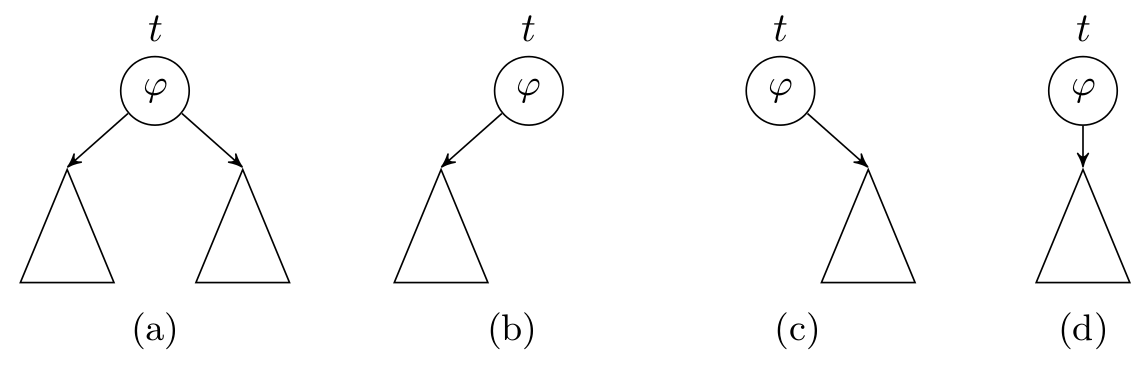
\includegraphics[width=0.9\textwidth]{figs/PTrees/ptrees.png}
%	%  \caption{Compact P-trees}
%	%\end{figure}
%
%	\begin{figure}[!ht]
%		\centering
%	  \begin{subfigure}[b]{0.3\textwidth}
%			\centering
%		  \begin{tikzpicture}[->,>=stealth',
%		    level1/.style={sibling distance=1.5cm}, level distance=35pt]
%		    \node [main node,inner sep=3pt,label={[xshift=0cm, yshift=0cm]$t$}] (1){$\varphi$}
%					child [edge from parent path ={(\tikzparentnode.-140) -- (\tikzchildnode.north)}] {
%						node [subtree,yshift=0.4cm] (2) {}}
%					child [edge from parent path ={(\tikzparentnode.-40) -- (\tikzchildnode.north)}] {
%						node [subtree,yshift=0.4cm] (3) {}};
%		  \end{tikzpicture}
%			\caption{\label{fig:compact1}}
%		\end{subfigure}%
%	  \begin{subfigure}[b]{0.2\textwidth}
%			\centering
%		  \begin{tikzpicture}[->,>=stealth',
%		    level1/.style={sibling distance=1.5cm}, level distance=35pt]
%			    \node [main node,inner sep=3pt,label={[xshift=0cm, yshift=0cm]$t$}] (1){$\varphi$}
%						child {node [subtree,yshift=0.4cm] (2) {}};
%		  \end{tikzpicture}
%			\caption{\label{fig:compact2}}
%		\end{subfigure}%
%	  \begin{subfigure}[b]{0.2\textwidth}
%			\centering
%			  \begin{tikzpicture}[->,>=stealth',
%			    level1/.style={sibling distance=1.5cm}, level distance=35pt]
%			    \node [main node,inner sep=3pt,label={[xshift=0cm, yshift=0cm]$t$}] (1){$\varphi$}
%						child [edge from parent path ={(\tikzparentnode.-140) -- (\tikzchildnode.north)}] {
%							node [subtree,yshift=0.4cm] (2) {}}
%		      		child {node [rectangle] (3) {} edge from parent[draw=none]
%			      };
%			  \end{tikzpicture}
%				\caption{\label{fig:compact3}}
%		\end{subfigure}%
%	  \begin{subfigure}[b]{0.2\textwidth}
%			\centering
%		  \begin{tikzpicture}[->,>=stealth',
%		    level1/.style={sibling distance=1.5cm}, level distance=35pt]
%			    \node [main node,inner sep=3pt,label={[xshift=0cm, yshift=0cm]$t$}] (1){$\varphi$}
%		      	child {node [rectangle] (2) {} edge from parent[draw=none]
%			      }
%						child [edge from parent path ={(\tikzparentnode.-40) -- (\tikzchildnode.north)}] {
%							node [subtree,yshift=0.4cm] (2) {}};
%		  \end{tikzpicture}
%			\caption{\label{fig:compact4}}
%		\end{subfigure}
%	  \caption{Compact P-trees}
%	%\vspace{-0.2cm}
%	  \label{fig:compact}
%	\end{figure}
%}

%\frameT{Relative Expressivity of Preference Languages}{
%	\begin{center}
%		Poss-theories = ASO-rules 
%		%$\subsetsim$ 
%		$\subset$
%			\dual{LP-trees/\dual{$\cap$/\dual{PLP-trees/\dual{$\cap$/P-trees}}}}
%			$\subset$ ASO-theories
%	\end{center}
%}
%
%\frameT{Computational Complexity Results}{
%	{\sc DomTest}: is it that $o \succeq_T o'$ in P-tree $T$?\\
%	{\sc OptTest}: is outcome $o$ optimal w.r.t $T$?\\
%	{\sc OptProp}: is there an optimal outcome $o$ w.r.t $T$ st $o \models \alpha$?
%	
%	\begin{figure}
%		\centering
%
%	  \begin{tabular}[0.5\textwidth]{ | c | c | c | c | }
%	    \hline
%	     & {\sc DomTest}& {\sc OptTest} & {\sc OptProp} \\
%			\hline
%			LP-tree & P & P & P \\
%			\hline
%			\pbox{20cm}{ASO-rule/ \\ Poss-theory} & P & coNP-c & $\deltap{2}$($P^{NP}$) \\
%	    \hline
%	    \tbf{P-tree} & \tbf{P} & \tbf{coNP-c}\fn{The complement problem is reduced from the SAT problem.}
%				& \tbf{$\deltap{2}$($P^{NP}$)-c}\fn{The problem is reduced from the Maximum Satisfying 
%																					Assignment (MSA) problem.}\\
%			\hline
%			ASO-theory & P & coNP-c & $\sigmap{2}$($NP^{NP}$)-c \\
%	    \hline
%			%ACP-net & NP-hard & P & P \\
%	    %\hline
%			%CCP-net & PSPACE-c & PSPACE-c? & PSPACE-c? \\
%	    %\hline
%	  \end{tabular}
%
%		\caption{Computational complexity results}
%
%	\end{figure}
%}

%\frameT{Computational Complexity Results}{
%	Dominance-testing ({\sc DomTest}): $o_1 \succ_T o_2$?\\
%	Optimality-testing ({\sc OptTest}): $o$ optimal w.r.t $T$?\\
%	Optimality-with-property ({\sc OptProp}): is there optimal $o$ 
%	with property $\alpha$?
%
%	\begin{enumerate}
%		\item {\sc DomTest}$\;\in P$
%		\item {\sc OptTest}$\;\in \coNP$-complete:
%			\begin{itemize}
%				\item The complement problem is reduced from the SAT problem.
%			\end{itemize}
%		\item {\sc OptProp}$\;\in \deltap{2}$-complete:
%			\begin{itemize}
%				\item The problem is reduced from the Maximum Satisfying Assignment (MSA) problem. 
%			\end{itemize}
%	\end{enumerate}
%}

%\frameT{Partial Lexicographic Preference Trees (PLP-Tree)}{
%	A \tit{PLP-tree} over $\CD(\cI)$ is a tree, where
%	\begin{enumerate}
%		\setlength\itemsep{0em}
%		\item every node $t$ is labeled with an attribute $\Attr(t)$ in $\cI$ and
%					a conditional preference table $\CPT(t)$,
%	  \item every non-leaf node $t$ has either one unlabeled outgoing edge or multiple
%					outgoing edges labeled, each labeled by some value in $\Dom(\Attr(t))$, and
%		\item every attribute appears \tit{at most} once on every branch.
%	\end{enumerate}
%}

\frameT{Example: The Cars Domain}{
  \begin{enumerate}
    \item \tbf{BodyType}(B): \{mvan, sedan, sport, suv\}.
    \item \tbf{Capacity}(C): \{2, 5, 7m\}.
    \item \tbf{Color}(O): \{black, blue, gray, red, white\}.
    \item \tbf{LuggageSize}(L): \{big, med, small\}.
    \item \tbf{Make}(M): \{bmw, ford, honda, vw\}.
    \item \tbf{Price}(P): \{low, med, high, vhigh\}.
    \item \tbf{Safety}(S): \{low, med, high\}.
  \end{enumerate}
}

\frameT{Partial Lexicographic Preference Trees (PLP-Trees)}{
	A \tit{PLP-tree} over $\CD(\cI)$ is a tree, where
	\begin{enumerate}
		\setlength\itemsep{0em}
		\item every non-leaf node $t$ is labeled with an attribute $\Attr(t)$ in $\cI$,
	  \item every non-leaf node $t$ has $|\Dom(\Attr(t))|$ outgoing edges labeled
					with a value of $\Attr(t)$, and
		\item every attribute appears \tit{at most} once on every branch.
	\end{enumerate}

	\begin{figure}[!ht]
	  \centering
      \begin{tikzpicture}[->,>=stealth',
	      level 1/.style={sibling distance=2cm, level distance=33pt},
	      level 2/.style={sibling distance=0.7cm, level distance=27pt}
	    ]
        \node [main node,inner sep=2pt] (1){S}
          child {node [main node,inner sep=2pt] (2) {C}
            child {node [rectangle,draw] (3) {} edge from parent node[left]  {\tiny{5}}}
            child {node [rectangle,draw] (4) {} edge from parent node[left]  {\tiny{7}}}
            child {node [rectangle,draw] (5) {} edge from parent node[right] {\tiny{2}}}
          edge from parent node[left] {\small{h}}}
          child {node [main node,inner sep=2pt] (6) {C}
            child {node [rectangle,draw] (7) {} edge from parent node[left]  {\tiny{5}}}
            child {node [rectangle,draw] (8) {} edge from parent node[left]  {\tiny{7}}}
            child {node [rectangle,draw] (9) {} edge from parent node[right] {\tiny{2}}}
          edge from parent node[left] {\small{m}}}
          child {node [main node,inner sep=2pt] (10) {C}
            child {node [rectangle,draw] (11) {} edge from parent node[left]  {\tiny{5}}}
            child {node [rectangle,draw] (12) {} edge from parent node[left]  {\tiny{7}}}
            child {node [rectangle,draw] (13) {} edge from parent node[right] {\tiny{2}}}
          edge from parent node[right] {\small{l}}};
      \end{tikzpicture}
	  \caption{A PLP-tree over cars}
	\end{figure}

\vspace{-1cm}

	\begin{center}
		{\transparent{0} Total preorder}
	\end{center}
}

\frameT{Partial Lexicographic Preference Trees (PLP-Trees)}{
	A \tit{PLP-tree} over $\CD(\cI)$ is a tree, where
	\begin{enumerate}
		\setlength\itemsep{0em}
		\item every non-leaf node $t$ is labeled with an attribute $\Attr(t)$ in $\cI$,
	  \item every non-leaf node $t$ has $|\Dom(\Attr(t))|$ outgoing edges labeled
					with a value of $\Attr(t)$, and
		\item every attribute appears \tit{at most} once on every branch.
	\end{enumerate}

	\begin{figure}[!ht]
	  \centering
      \begin{tikzpicture}[->,>=stealth',
	      level 1/.style={sibling distance=2cm, level distance=33pt},
	      level 2/.style={sibling distance=0.7cm, level distance=27pt}
	    ]
        \node [main node,inner sep=2pt] (1){S}
          child {node [main node,inner sep=2pt] (2) {C}
            child {node [rectangle,draw] (3) {} edge from parent node[left]  {\tiny{5}}}
            child {node [rectangle,draw] (4) {} edge from parent node[left]  {\tiny{7}}}
            child {node [rectangle,draw] (5) {} edge from parent node[right] {\tiny{2}}}
          edge from parent node[left] {\small{h}}}
          child {node [main node,inner sep=2pt] (6) {C}
            child {node [rectangle,draw] (7) {} edge from parent node[left]  {\tiny{5}}}
            child {node [rectangle,draw] (8) {} edge from parent node[left]  {\tiny{7}}}
            child {node [rectangle,draw] (9) {} edge from parent node[right] {\tiny{2}}}
          edge from parent node[left] {\small{m}}}
          child {node [main node,inner sep=2pt] (10) {C}
            child {node [rectangle,draw] (11) {} edge from parent node[left]  {\tiny{5}}}
            child {node [rectangle,draw] (12) {} edge from parent node[left]  {\tiny{7}}}
            child {node [rectangle,draw] (13) {} edge from parent node[right] {\tiny{2}}}
          edge from parent node[right] {\small{l}}};
      \end{tikzpicture}
	  \caption{A PLP-tree over cars}
	\end{figure}

\vspace{-1cm}

	\begin{center}
		Total preorder
	\end{center}
}

\frameT{Partial Lexicographic Preference Trees (PLP-Trees)}{
  \begin{figure}[ht!]
    \centering
      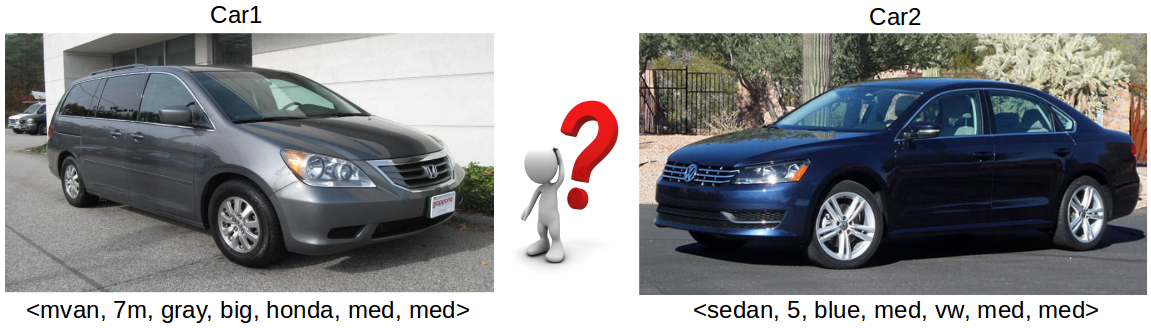
\includegraphics[width=0.95\textwidth]{figs/Cars/individual.png}
  \end{figure}

\vspace{-0.5cm}

	\begin{figure}[!ht]
	  \centering
      \begin{tikzpicture}[->,>=stealth',
	      level 1/.style={sibling distance=2cm, level distance=33pt},
	      level 2/.style={sibling distance=0.7cm, level distance=27pt}
	    ]
        \node [main node,inner sep=2pt] (1){S}
          child {node [main node,inner sep=2pt] (2) {C}
            child {node [rectangle,draw] (3) {} edge from parent node[left]  {\tiny{5}}}
            child {node [rectangle,draw] (4) {} edge from parent node[left]  {\tiny{7}}}
            child {node [rectangle,draw] (5) {} edge from parent node[right] {\tiny{2}}}
          edge from parent node[left] {\small{h}}}
          child {node [main node,inner sep=2pt] (6) {C}
            child [green] {node [rectangle,draw] (7) {} edge from parent node[left]  {\tiny{5}}}
            child [red] {node [rectangle,draw] (8) {} edge from parent node[left]  {\tiny{7}}}
            child {node [rectangle,draw] (9) {} edge from parent node[right] {\tiny{2}}}
          edge from parent node[left] {\small{m}}}
          child {node [main node,inner sep=2pt] (10) {C}
            child {node [rectangle,draw] (11) {} edge from parent node[left]  {\tiny{5}}}
            child {node [rectangle,draw] (12) {} edge from parent node[left]  {\tiny{7}}}
            child {node [rectangle,draw] (13) {} edge from parent node[right] {\tiny{2}}}
          edge from parent node[right] {\small{l}}};
      \end{tikzpicture}
	  \caption{A PLP-tree over cars}
	\end{figure}

\vspace{-1cm}

	\begin{center}
		$\textcolor{green}{Car2} \succ \textcolor{red}{Car1}$
	\end{center}
}

\frameT{Compact Representations of PLP-Tree}{
	\begin{figure}
	  \centering
		\begin{subfigure}[b]{0.65\textwidth}
	    \centering
      \begin{tikzpicture}[->,>=stealth',
	      level 1/.style={sibling distance=2cm, level distance=33pt},
	      level 2/.style={sibling distance=0.7cm, level distance=27pt}
	    ]
        \node [main node,inner sep=2pt] (1){S}
          child {node [main node,inner sep=2pt] (2) {C}
            child {node [rectangle,draw] (3) {} edge from parent node[left]  {\tiny{5}}}
            child {node [rectangle,draw] (4) {} edge from parent node[left]  {\tiny{7}}}
            child {node [rectangle,draw] (5) {} edge from parent node[right] {\tiny{2}}}
          edge from parent node[left] {\small{h}}}
          child {node [main node,inner sep=2pt] (6) {C}
            child {node [rectangle,draw] (7) {} edge from parent node[left]  {\tiny{5}}}
            child {node [rectangle,draw] (8) {} edge from parent node[left]  {\tiny{7}}}
            child {node [rectangle,draw] (9) {} edge from parent node[right] {\tiny{2}}}
          edge from parent node[left] {\small{m}}}
          child {node [main node,inner sep=2pt] (10) {C}
            child {node [rectangle,draw] (11) {} edge from parent node[left]  {\tiny{5}}}
            child {node [rectangle,draw] (12) {} edge from parent node[left]  {\tiny{7}}}
            child {node [rectangle,draw] (13) {} edge from parent node[right] {\tiny{2}}}
          edge from parent node[right] {\small{l}}};
      \end{tikzpicture}
			\caption{Full}
		\end{subfigure}
		\begin{subfigure}[b]{0.25\textwidth}
			\centering
      \begin{tikzpicture}[->,>=stealth',
	      level 1/.style={sibling distance=2cm, level distance=33pt},
	      level 2/.style={sibling distance=0.7cm, level distance=27pt}
	    ]
	  	      
	  	  \node[main node,inner sep=2pt] (1) {S};
	  	  \node[rectangle,draw,inner sep=2pt] at (1,0) {$h\!\! >\!\! m\!\! >\!\! l$};
	
	  	  \node[main node,inner sep=2pt] (2) [below of=1] {C};
	  	  \node[rectangle,draw,inner sep=2pt] at (1,-1) {$5 \!\!>\!\! 7\!\!>\!\! 2$};
	  	
	  	  \node[rectangle] (3) [below of=2] {};

	  	  \path[every node/.style={font=\sffamily\small}]
	  	    (1) edge (2);
	  	\end{tikzpicture}
			\caption{Compact}
		\end{subfigure}
	\caption{Unconditional Importance \& Unconditional Preference (UIUP)}
	\end{figure}
}

\frameT{Compact Representations of PLP-Tree}{
	\begin{figure}
	  \centering
		\begin{subfigure}[b]{0.65\textwidth}
	    \centering
      \begin{tikzpicture}[->,>=stealth',
	      level 1/.style={sibling distance=2cm, level distance=33pt},
	      level 2/.style={sibling distance=0.7cm, level distance=27pt}
	    ]
        \node [main node,inner sep=2pt] (1){S}
          child {node [main node,inner sep=2pt] (2) {C}
            child {node [rectangle,draw] (3) {} edge from parent node[left]  {\tiny{5}}}
            child {node [rectangle,draw] (4) {} edge from parent node[left]  {\tiny{7}}}
            child {node [rectangle,draw] (5) {} edge from parent node[right] {\tiny{2}}}
          edge from parent node[left] {\small{h}}}
          child {node [main node,inner sep=2pt] (6) {C}
            child {node [rectangle,draw] (7) {} edge from parent node[left]  {\tiny{7}}}
            child {node [rectangle,draw] (8) {} edge from parent node[left]  {\tiny{5}}}
            child {node [rectangle,draw] (9) {} edge from parent node[right] {\tiny{2}}}
          edge from parent node[left] {\small{m}}}
          child {node [main node,inner sep=2pt] (10) {C}
            child {node [rectangle,draw] (11) {} edge from parent node[left]  {\tiny{2}}}
            child {node [rectangle,draw] (12) {} edge from parent node[left]  {\tiny{5}}}
            child {node [rectangle,draw] (13) {} edge from parent node[right] {\tiny{7}}}
          edge from parent node[right] {\small{l}}};
      \end{tikzpicture}
			\caption{Full}
		\end{subfigure}
		\begin{subfigure}[b]{0.25\textwidth}
			\centering
      \begin{tikzpicture}[->,>=stealth',
	      level 1/.style={sibling distance=2cm, level distance=33pt},
	      level 2/.style={sibling distance=0.7cm, level distance=27pt}
	    ]
	  	      
	  	  \node[main node,inner sep=2pt] (1) {S};
	  	  \node[rectangle,draw,inner sep=2pt] at (1,0) {$h\!\! >\!\! m\!\! >\!\! l$};
	
	  	  \node[main node,inner sep=2pt] (2) [below of=1] {C};
	    	\node[rectangle split, rectangle split parts=3, draw,inner sep=2pt,font=\sffamily\small] at (1.2,-1.3)
	    	    {
							$h\!:\!5 \!\!>\!\! 7\!\!>\!\! 2$
	    	      \nodepart{second}
							$m\!:\!7 \!\!>\!\! 5\!\!>\!\! 2$
	    	      \nodepart{third}
							$l\!:\!2 \!\!>\!\! 5\!\!>\!\! 7$
	    	    };
	  	
	  	  \node[rectangle] (3) [below of=2] {};

	  	  \path[every node/.style={font=\sffamily\small}]
	  	    (1) edge (2);
	  	\end{tikzpicture}
			\caption{Compact}
		\end{subfigure}
	\caption{Unconditional Importance \& Conditional Preference (UICP)}
	\end{figure}
}

\frameT{Compact Representations of PLP-Tree}{
	\begin{figure}
	  \centering
		\begin{subfigure}[b]{0.95\textwidth}
	    \centering
      \begin{tikzpicture}[->,>=stealth',
	      level 1/.style={sibling distance=2.9cm, level distance=33pt},
	      level 2/.style={sibling distance=1.8cm, level distance=27pt},
	      level 3/.style={sibling distance=0.7cm, level distance=27pt}
	    ]
        \node [main node,inner sep=2pt] (1){S}
          child {node [main node,inner sep=2pt] (2) {C}
            child {node [main node,inner sep=2pt] (3) {L}
            	child {node [rectangle,draw] (14) {} edge from parent node[left]  {\tiny{b}}}
            	child {node [rectangle,draw] (15) {} edge from parent node[left]  {\tiny{m}}}
            	child {node [rectangle,draw] (16) {} edge from parent node[right] {\tiny{s}}}
						edge from parent node[left]  {\tiny{5}}}
            child {node [main node,inner sep=2pt] (4) {L}
            	child {node [rectangle,draw] (17) {} edge from parent node[left]  {\tiny{b}}}
            	child {node [rectangle,draw] (18) {} edge from parent node[left]  {\tiny{m}}}
            	child {node [rectangle,draw] (19) {} edge from parent node[right] {\tiny{s}}}
						edge from parent node[left]  {\tiny{7}}}
            child {node [main node,inner sep=2pt] (5) {L}
            	child {node [rectangle,draw] (20) {} edge from parent node[left]  {\tiny{b}}}
            	child {node [rectangle,draw] (21) {} edge from parent node[left]  {\tiny{m}}}
            	child {node [rectangle,draw] (22) {} edge from parent node[right] {\tiny{s}}}
						edge from parent node[left]  {\tiny{2}}}
          edge from parent node[left] {\small{h}}}
          child {node [rectangle,draw] (6) {} edge from parent node[left] {\small{m}}}
          child {node [main node,inner sep=2pt] (10) {L}
            child {node [main node,inner sep=2pt] (11) {C} 
            	child {node [rectangle,draw] (23) {} edge from parent node[left]  {\tiny{5}}}
            	child {node [rectangle,draw] (24) {} edge from parent node[left]  {\tiny{7}}}
            	child {node [rectangle,draw] (25) {} edge from parent node[right] {\tiny{2}}}
						edge from parent node[left]  {\tiny{b}}}
            child {node [main node,inner sep=2pt] (12) {C} 
            	child {node [rectangle,draw] (26) {} edge from parent node[left]  {\tiny{5}}}
            	child {node [rectangle,draw] (27) {} edge from parent node[left]  {\tiny{7}}}
            	child {node [rectangle,draw] (28) {} edge from parent node[right] {\tiny{2}}}
						edge from parent node[left]  {\tiny{m}}}
            child {node [main node,inner sep=2pt] (13) {C} 
            	child {node [rectangle,draw] (29) {} edge from parent node[left]  {\tiny{5}}}
            	child {node [rectangle,draw] (30) {} edge from parent node[left]  {\tiny{7}}}
            	child {node [rectangle,draw] (31) {} edge from parent node[right] {\tiny{2}}}
						edge from parent node[left]  {\tiny{s}}}
          edge from parent node[right] {\small{l}}};
      \end{tikzpicture}
			\caption{Full}
		\end{subfigure}\\
		\begin{subfigure}[b]{0.35\textwidth}
			\centering
      \begin{tikzpicture}[->,>=stealth',
	      level 1/.style={sibling distance=2cm, level distance=33pt},
	      level 2/.style={sibling distance=0.7cm, level distance=27pt}
	    ]
	  	      
	  	  \node[main node,inner sep=2pt] (1) {S};
	  	  \node[rectangle,draw,inner sep=2pt] at (1,0) {$h\!\! >\!\! m\!\! >\!\! l$};
	
	  	  \node[main node,inner sep=2pt] (2) [below left of=1] {C};
	  	  \node[rectangle,draw,inner sep=2pt] at (-1.6,-0.7) {$5\!\! >\!\! 7\!\! >\!\! 2$};

	  	  \node[main node,inner sep=2pt] (3) [below of=2] {L};
	  	  \node[rectangle,draw,inner sep=2pt] at (-1.6,-1.7) {$b\!\! >\!\! m\!\! >\!\! s$};
	  	
	  	  \node[main node,inner sep=2pt] (4) [below right of=1] {L};
	  	  \node[rectangle,draw,inner sep=2pt] at (1.6,-0.7) {$b\!\! >\!\! m\!\! >\!\! s$};
	  	
	  	  \node[main node,inner sep=2pt] (5) [below of=4] {C};
	  	  \node[rectangle,draw,inner sep=2pt] at (1.6,-1.7) {$5\!\! >\!\! 7\!\! >\!\! 2$};

	  	  %\node[rectangle] (6) [below of=5] {};

	  	  \path[every node/.style={font=\sffamily\small}]
	  	    (1) edge [left]  node{\tiny h} (2)
	  	    (1) edge [right] node{\tiny l} (4)
	  	    (2) edge (3)
	  	    (4) edge (5);
	  	\end{tikzpicture}
			\caption{Compact}
		\end{subfigure}
	\caption{Conditional Importance \& Unconditional Preference (CIUP)}
	\end{figure}
}

\frameT{Compact Representations of PLP-Tree}{
	\begin{figure}
	  \centering
		\begin{subfigure}[b]{0.95\textwidth}
	    \centering
      \begin{tikzpicture}[->,>=stealth',
	      level 1/.style={sibling distance=2.9cm, level distance=33pt},
	      level 2/.style={sibling distance=1.8cm, level distance=27pt},
	      level 3/.style={sibling distance=0.7cm, level distance=27pt}
	    ]
        \node [main node,inner sep=2pt] (1){S}
          child {node [main node,inner sep=2pt] (2) {C}
            child {node [main node,inner sep=2pt] (3) {L}
            	child {node [rectangle,draw] (14) {} edge from parent node[left]  {\tiny{m}}}
            	child {node [rectangle,draw] (15) {} edge from parent node[left]  {\tiny{b}}}
            	child {node [rectangle,draw] (16) {} edge from parent node[right] {\tiny{s}}}
						edge from parent node[left]  {\tiny{5}}}
            child {node [main node,inner sep=2pt] (4) {L}
            	child {node [rectangle,draw] (17) {} edge from parent node[left]  {\tiny{b}}}
            	child {node [rectangle,draw] (18) {} edge from parent node[left]  {\tiny{m}}}
            	child {node [rectangle,draw] (19) {} edge from parent node[right] {\tiny{s}}}
						edge from parent node[left]  {\tiny{7}}}
            child {node [main node,inner sep=2pt] (5) {L}
            	child {node [rectangle,draw] (20) {} edge from parent node[left]  {\tiny{s}}}
            	child {node [rectangle,draw] (21) {} edge from parent node[left]  {\tiny{m}}}
            	child {node [rectangle,draw] (22) {} edge from parent node[right] {\tiny{b}}}
						edge from parent node[left]  {\tiny{2}}}
          edge from parent node[left] {\small{h}}}
          child {node [rectangle,draw] (6) {} edge from parent node[left] {\small{m}}}
          child {node [main node,inner sep=2pt] (10) {L}
            child {node [main node,inner sep=2pt] (11) {C} 
            	child {node [rectangle,draw] (23) {} edge from parent node[left]  {\tiny{7}}}
            	child {node [rectangle,draw] (24) {} edge from parent node[left]  {\tiny{5}}}
            	child {node [rectangle,draw] (25) {} edge from parent node[right] {\tiny{2}}}
						edge from parent node[left]  {\tiny{b}}}
            child {node [main node,inner sep=2pt] (12) {C} 
            	child {node [rectangle,draw] (26) {} edge from parent node[left]  {\tiny{5}}}
            	child {node [rectangle,draw] (27) {} edge from parent node[left]  {\tiny{7}}}
            	child {node [rectangle,draw] (28) {} edge from parent node[right] {\tiny{2}}}
						edge from parent node[left]  {\tiny{m}}}
            child {node [main node,inner sep=2pt] (13) {C} 
            	child {node [rectangle,draw] (29) {} edge from parent node[left]  {\tiny{2}}}
            	child {node [rectangle,draw] (30) {} edge from parent node[left]  {\tiny{5}}}
            	child {node [rectangle,draw] (31) {} edge from parent node[right] {\tiny{7}}}
						edge from parent node[left]  {\tiny{s}}}
          edge from parent node[right] {\small{l}}};
      \end{tikzpicture}
			\caption{Full}
		\end{subfigure}\\
		\begin{subfigure}[b]{0.4\textwidth}
			\centering
      \begin{tikzpicture}[->,>=stealth',
	      level 1/.style={sibling distance=2cm, level distance=33pt},
	      level 2/.style={sibling distance=0.7cm, level distance=27pt}
	    ]
	  	      
	  	  \node[main node,inner sep=2pt] (1) {S};
	  	  \node[rectangle,draw,inner sep=2pt] at (1,0) {$h\!\! >\!\! m\!\! >\!\! l$};
	
	  	  \node[main node,inner sep=2pt] (2) [below left of=1] {C};
	  	  \node[rectangle,draw,inner sep=2pt] at (-1.6,-0.7) {$5\!\! >\!\! 7\!\! >\!\! 2$};

	  	  \node[main node,inner sep=2pt] (3) [below of=2] {L};
	    	\node[rectangle split, rectangle split parts=3, draw,inner sep=2pt,font=\sffamily\small] at (-1.8,-1.7)
	    	    {
							$2\!:\!s \!\!>\!\! m\!\!>\!\! b$
	    	      \nodepart{second}
							$5\!:\!m \!\!>\!\! b\!\!>\!\! s$
	    	      \nodepart{third}
							$7\!:\!b \!\!>\!\! m\!\!>\!\! s$
	    	    };
	  	
	  	  \node[main node,inner sep=2pt] (4) [below right of=1] {L};
	  	  \node[rectangle,draw,inner sep=2pt] at (1.6,-0.7) {$b\!\! >\!\! m\!\! >\!\! s$};
	  	
	  	  \node[main node,inner sep=2pt] (5) [below of=4] {C};
	    	\node[rectangle split, rectangle split parts=3, draw,inner sep=2pt,font=\sffamily\small] at (1.8,-1.7)
	    	    {
							$b\!:\!7 \!\!>\!\! 5\!\!>\!\! 2$
	    	      \nodepart{second}
							$m\!:\!5 \!\!>\!\! 7\!\!>\!\! 2$
	    	      \nodepart{third}
							$s\!:\!2 \!\!>\!\! 5\!\!>\!\! 7$
	    	    };

	  	  %\node[rectangle] (6) [below of=5] {};

	  	  \path[every node/.style={font=\sffamily\small}]
	  	    (1) edge [left]  node{\tiny h} (2)
	  	    (1) edge [right] node{\tiny l} (4)
	  	    (2) edge (3)
	  	    (4) edge (5);
	  	\end{tikzpicture}
			\caption{Compact}
		\end{subfigure}
	\vspace{-0.2cm}
	\caption{Conditional Importance \& Conditional Preference (CICP)}
	\end{figure}
}

\frameT{Lexicographic Preference Trees (LP-Trees)}
{
  \begin{enumerate}
    \item An \tit{LP-tree} $\cL$ over $\CD(\cI)$ is a PLP-tree, where
    \begin{itemize}
      \item each attribute appears \tbf{exactly once} on every path from the root to a leaf.
			\item Unlike PLP-trees, an LP-tree induces a total order.
    \end{itemize}
  \end{enumerate}
}
